\documentclass[14pt]{extarticle}
\usepackage{fontspec}
\usepackage{geometry}
\geometry{a4paper, margin=2.1cm}
\usepackage{graphicx}
\usepackage{booktabs}
\usepackage{array}
\usepackage{longtable}
\usepackage{amsmath}
\usepackage{amssymb}
\usepackage[table]{xcolor}
\usepackage{titlesec}
\usepackage{fancyhdr}
\renewcommand{\contentsname}{\color{theme}สารบัญ}
\usepackage{enumitem}
\usepackage[most]{tcolorbox}
\usepackage{hyperref}

\definecolor{theme}{HTML}{2b6a77}
\definecolor{themeD}{HTML}{1f4e58}
\definecolor{ink}{HTML}{232d33}
\definecolor{ok}{HTML}{3f8161}
\definecolor{warn}{HTML}{b5651d}
\definecolor{cardbg}{HTML}{f3f6f7}
\definecolor{softgray}{HTML}{eef1f2}
\hypersetup{colorlinks=true, linkcolor=theme, urlcolor=theme, pdftitle={SPR Fracture Detection - Phase 1 Final Report}}

\setmainfont{THSarabunNew.ttf}[
  Path=./fonts/, BoldFont=THSarabunNew Bold.ttf,
  ItalicFont=THSarabunNew Italic.ttf, BoldItalicFont=THSarabunNew BoldItalic.ttf]
\setmonofont{cour.ttf}[Path=./fonts/, BoldFont=courbd.ttf, Scale=0.82]
\XeTeXlinebreaklocale "th"
\XeTeXlinebreakskip = 0pt plus 0.1pt

\titleformat{\section}{\Large\bfseries\color{theme}}{\thesection.}{0.5em}{}
\titleformat{\subsection}{\large\bfseries\color{ink}}{\thesubsection}{0.5em}{}
\setlist{itemsep=1pt, topsep=2pt}
\pagestyle{fancy}\fancyhf{}
\fancyhead[L]{\small\color{ink} SPR Fracture Detection --- Phase 1 Final Report}
\fancyhead[R]{\small\color{ink}\thepage}
\renewcommand{\headrulewidth}{0.4pt}
\renewcommand{\headrule}{\hbox to\headwidth{\color{theme!45}\leaders\hrule height \headrulewidth\hfill}}
\newcommand{\code}[1]{{\ttfamily\detokenize{#1}}}
\newcommand{\pgood}{\textcolor{ok}{$\boxtimes$}}
\newcommand{\ppart}{\textcolor{warn}{$\sim$}}
\newtcolorbox{keybox}{colback=cardbg, colframe=theme!55, boxrule=0.8pt, arc=2pt, left=8pt, right=8pt, top=5pt, bottom=6pt}
\newtcolorbox{verdictbox}[1]{colback=cardbg, colframe=theme, boxrule=1pt, arc=2pt, left=8pt, right=8pt, top=4pt, bottom=5pt, title=#1, coltitle=white, colbacktitle=theme, fonttitle=\bfseries\small}

\begin{document}

% ================= TITLE =================
\begin{center}
{\color{theme}\rule{\linewidth}{2.5pt}}\\[8pt]
{\LARGE\bfseries\color{themeD} การตรวจจับรอยแตกกระดูกเชิงกรานระดับต่ำกว่ามิลลิเมตร\\[3pt]
ด้วยลายเซ็นการกระเจิงรังสีเอกซ์ (Scatter-to-Primary Ratio)}\\[8pt]
{\Large\color{theme} รายงานฉบับสมบูรณ์ --- Phase 1 (Feasibility Study)}\\[6pt]
{\large การจำลอง Monte Carlo ด้วย OpenGATE 10 / Geant4}\\[4pt]
{\small Baanwit Academy \quad$\bullet$\quad repository: \code{intraprasart/GATE-Xray-pelvis-SPR} \quad$\bullet$\quad \today}\\[6pt]
{\color{theme}\rule{\linewidth}{2.5pt}}
\end{center}
\vspace{6pt}

% ================= ABSTRACT =================
\begin{keybox}
\textbf{\color{themeD} บทคัดย่อ.}\ โครงการนี้ทดสอบสมมติฐานว่ารอยแตกกระดูกทิ้ง ``ลายเซ็น'' ที่ตรวจจับได้ใน
อัตราส่วนการกระเจิงต่อรังสีปฐมภูมิ (SPR) ของภาพรังสีเอกซ์ ผ่านการจำลอง Monte Carlo โดยพัฒนาระเบียบวิธี
ที่แยกสัญญาณของรอยแตกออกจากปัจจัยรบกวนอย่างเข้มงวด (\textit{matched control} + \textit{multi-seed
significance} + a-priori ROI) แล้วทดสอบผ่าน 6 เสาหลัก ผลสรุป: \textbf{สมมติฐานหลักได้รับการสนับสนุน
อย่างแข็งแรง} --- SPR มีลายเซ็นรอยแตกที่ \textbf{ตรวจพบได้จริง} (ทั้ง 4 ขนาด, $p<0.02$),
\textbf{ยืนยันเชิงสถิติ} (รอยแตกเล็กสุด 0.306~มม.\ ยืนยันที่ $p=4\times10^{-5}$), \textbf{ไม่ใช่ artifact}
(false-positive rate $\approx5\%$), และ\textbf{มีที่มาเชิงฟิสิกส์} (สัญญาณแรงขึ้นที่พลังงานต่ำ + baseline SPR
ลดลง monotonic ตามพลังงาน) อย่างไรก็ตามพบขอบเขตที่ชัดเจน: \textbf{SPR ไวต่อ ``การมีอยู่'' ของรอยแตก
มากกว่า ``ความกว้าง''} (สัญญาณอิ่มตัวเกิน $\sim$0.5~มม.) และการทดสอบเชิงกลไก (พลังงาน/มุม) ยัง
ไม่สมบูรณ์เชิงปริมาณที่จำนวน seed ปัจจุบัน โดยรวมเป็น \textbf{proof-of-concept ที่มั่นคง}สำหรับการพัฒนาต่อ
\end{keybox}

{\small\tableofcontents}
\vspace{4pt}

% ================= 1. INTRO =================
\section{บทนำและวัตถุประสงค์}
รอยแตกกระดูกแบบเส้นผม (hairline / sub-millimetre fracture) มักตรวจพบได้ยากในภาพรังสีทั่วไป เนื่องจากความ
แตกต่างของการดูดกลืนรังสี (attenuation) ที่รอยแตกสร้างขึ้นมีค่าน้อยมาก \textbf{สมมติฐานหลัก}ของโครงการคือ
รอยแตกทำให้เกิดการเปลี่ยนแปลงเฉพาะจุดขององค์ประกอบการกระเจิงรังสี ซึ่งวัดผ่าน
\[ \mathrm{SPR}(x,y)=\frac{I_{\text{scatter}}(x,y)}{I_{\text{primary}}(x,y)} \]
และอาจให้ ``ลายเซ็น'' ที่ตรวจจับได้ดีกว่าการดูดกลืนโดยตรง

\noindent\textbf{วัตถุประสงค์ Phase 1:} ทดสอบว่าลายเซ็น SPR จากรอยแตก (1)~ตรวจพบได้, (2)~ยืนยันเชิงสถิติ,
(3)~ไม่ใช่ artifact ของระเบียบวิธี, (4)~มีที่มาเชิงฟิสิกส์ และ (5)~ระบุขอบเขตความสามารถ --- ผ่านการจำลอง
Monte Carlo โดยใช้เพียงโมเดลที่มีอยู่ (รอยแตก 4 ขนาด) แล้วปรับพารามิเตอร์การรัน

% ================= 2. METHODS =================
\section{ระเบียบวิธี}

\subsection{การจำลองด้วย Monte Carlo}
ใช้ OpenGATE 10 (Geant4, \code{G4EmLivermorePhysics}) จำลองภาพรังสีเชิงกรานแบบ AP; แหล่งกำเนิดแกมมา
mono 80~keV (ยกเว้นการกวาดพลังงาน); วัสดุ \code{G4_BONE_COMPACT_ICRU}; SOD 800~มม., ODD 400~มม.
แบบจำลองแยกโฟตอนที่ระนาบฉากรับเป็นปฐมภูมิ/กระเจิง (จากมุมเบี่ยง $\le0.5^\circ$ และ $|E-E_0|\le1$~keV)
แล้วคำนวณแผนที่ SPR; รอยแตก 4 ขนาด: ช่องว่าง 0.306 / 0.43 / 0.54 / 1.0~มม.

\subsection{Matched control --- ตัด confound ของ mesh (จุดสำคัญ)}
การวิเคราะห์เบื้องต้นพบว่าการเทียบโมเดล ``ปกติ'' กับ ``รอยแตก'' ที่เป็น\textbf{คนละ mesh กัน} ทำให้ผลต่าง
$\Delta\mathrm{SPR}$ ถูกครอบงำด้วยความต่างของ tessellation ทั้งก้อน มิใช่รอยแตก จึงสร้าง
\textbf{matched control} = mesh เดียวกับ fracture แต่ ``ถม'' ร่องด้วยกระดูก (boolean union) ผ่านการตรวจสอบว่า
control กับ fracture ตรงกันทุกจุด\textbf{นอกบริเวณร่อง} (คลาดเคลื่อน 0.0000~มม.\ จากจุดยอด $>$349{,}000 จุด)
$\Rightarrow$ $\Delta\mathrm{SPR}=\mathrm{SPR}_{\text{fracture}}-\mathrm{SPR}_{\text{control}}$
\textbf{แยกเฉพาะผลของรอยแตกล้วน ๆ}

\subsection{Multi-seed significance + a-priori ROI}
รันกระบวนการซ้ำด้วยเมล็ดสุ่มอิสระ $N$ ชุด (control+fracture ใช้ seed เดียวกันต่อ realization = common random
numbers) แล้วทดสอบว่าค่าเฉลี่ย $\Delta\mathrm{SPR}$ ที่ ROI ต่างจาก 0 หรือไม่:
\[ t=\frac{\overline{\Delta\mathrm{SPR}}}{s/\sqrt{N}},\qquad \mathrm{df}=N-1 \]
โดยกำหนด ROI 16$\times$16~พิกเซล ที่ตำแหน่งร่อง\textbf{ก่อนดูผล} (a-priori) เทียบกับ background ROI;
\textbf{บีบลำแสง (collimation, field 40~มม.)} เพื่อเพิ่มโฟตอน/พิกเซล ($\sim$3{,}600) ที่บริเวณร่อง

\subsection{ระบบคำนวณ}
พัฒนาระบบงานทางไกล (job server + worker) ที่กระจายงานแบบ multi-process (sharding) และรองรับการสั่งงาน
ผ่านเซิร์ฟเวอร์ ทำให้ทำ parameter sweep ได้อย่างเป็นระบบและทำซ้ำได้ --- การทดลองทั้งหมดในรายงานนี้รันบน
ระบบดังกล่าว

% ================= 3. RESULTS =================
\section{ผลการดำเนินการ (6 เสาหลัก)}

\subsection{การตรวจพบ (CL-0)}
ที่ 8 seeds ต่อขนาด: ตรวจพบรอยแตก\textbf{ครบทั้ง 4 ขนาด} ($p<0.02$ ทุกขนาด) โดย $\Delta\mathrm{SPR}<0$
(ช่องอากาศ $\to$ primary ทะลุมากขึ้น $\to$ SPR ต่ำลง --- สอดคล้องฟิสิกส์) และ background ROI เป็น null
(สัญญาณเฉพาะที่ร่อง) สัญญาณโตในช่วง 0.306$\to$0.54~มม.\ แล้วเข้าสู่ระดับอิ่มตัว

\begin{table}[h]\centering\small
\renewcommand{\arraystretch}{1.2}
\begin{tabular}{c c c c c}
\rowcolor{softgray} ขนาดร่อง & $\Delta$SPR (ROI) & $|t|$ & $p$ & background \\
\midrule
0.306 มม. & $-3.3\times10^{-5}$ & 3.12 & 0.017 & null \\
0.43 มม.\  & $-3.4\times10^{-5}$ & 3.66 & 0.008 & null \\
0.54 มม.\  & $-4.9\times10^{-5}$ & 4.84 & 0.002 & null \\
1.0 มม.\   & $-4.2\times10^{-5}$ & 4.32 & 0.004 & null \\
\bottomrule
\end{tabular}
\end{table}
\vspace{-2pt}
\noindent นอกจากนี้พบว่า\textbf{ตัวชี้วัดเชิงพื้นผิว (local variance, entropy) ตรวจไม่พบสัญญาณ} เพราะรอยแตก
ทำให้ SPR เลื่อนระดับแบบสม่ำเสมอ (mean shift) ซึ่งตัวชี้วัดความแปรปรวน invariant โดยธรรมชาติ
($\mathrm{STD}(x+c)=\mathrm{STD}(x)$) $\Rightarrow$ \textbf{observable ที่ถูกต้องคือระดับ SPR เอง}

\begin{figure}[h]\centering
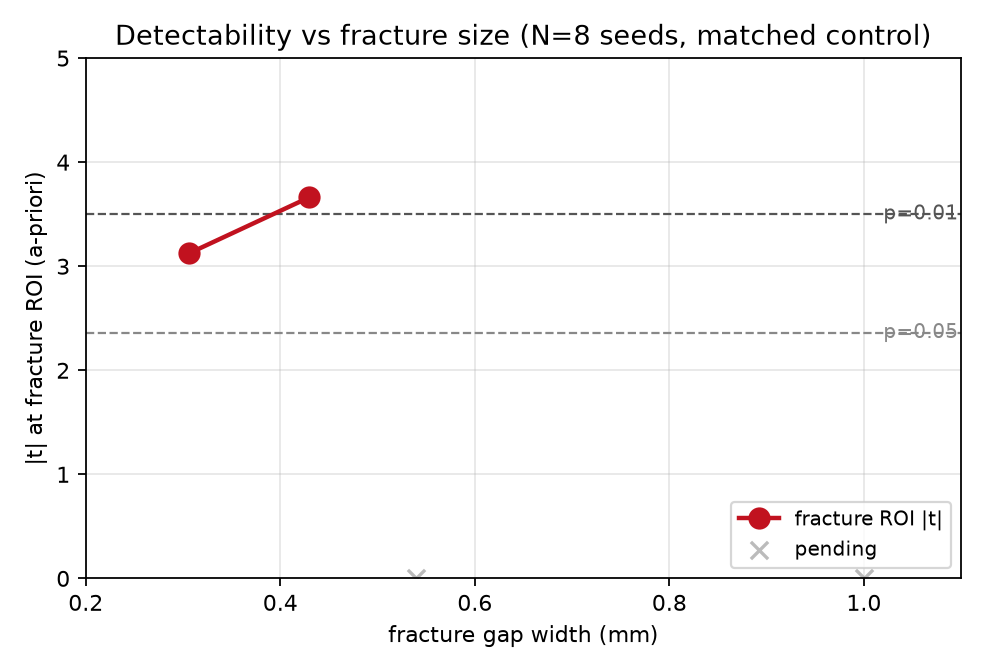
\includegraphics[width=0.86\textwidth]{fig/trend.png}
\caption{เส้นโค้ง detectability: ความแรง $|t|$ (ซ้าย) และขนาดสัญญาณ $|\Delta$SPR$|$ (ขวา) เทียบขนาดรอยแตก ---
ขึ้นในช่วง 0.3--0.5~มม.\ แล้วอิ่มตัว}
\end{figure}

\subsection{ความ robust และกำลังทางสถิติ (CL-1)}
Bootstrap 95\% CI ของ $\Delta\mathrm{SPR}$ \textbf{ตัดค่า 0 ทุกขนาด} (การตรวจพบไม่ใช่ความบังเอิญ) แต่รอยแตก
เล็กสุด (0.306~มม.) ยัง\textbf{ก้ำกึ่ง}ที่ $N=8$ (ความน่าเชื่อถือ 80\%) การวิเคราะห์กำลังชี้ว่าต้องการ $\sim$13 seeds
เพื่อยืนยันที่ $p<0.01$ --- \textbf{จึงรันยืนยันจริงที่ $N=30$ ได้ผล $p=0.00004$ ($t=-4.86$, reliability 99\%)}
ยืนยันการตรวจพบรอยแตกเล็กสุดอย่างเด็ดขาด

\begin{figure}[h]\centering
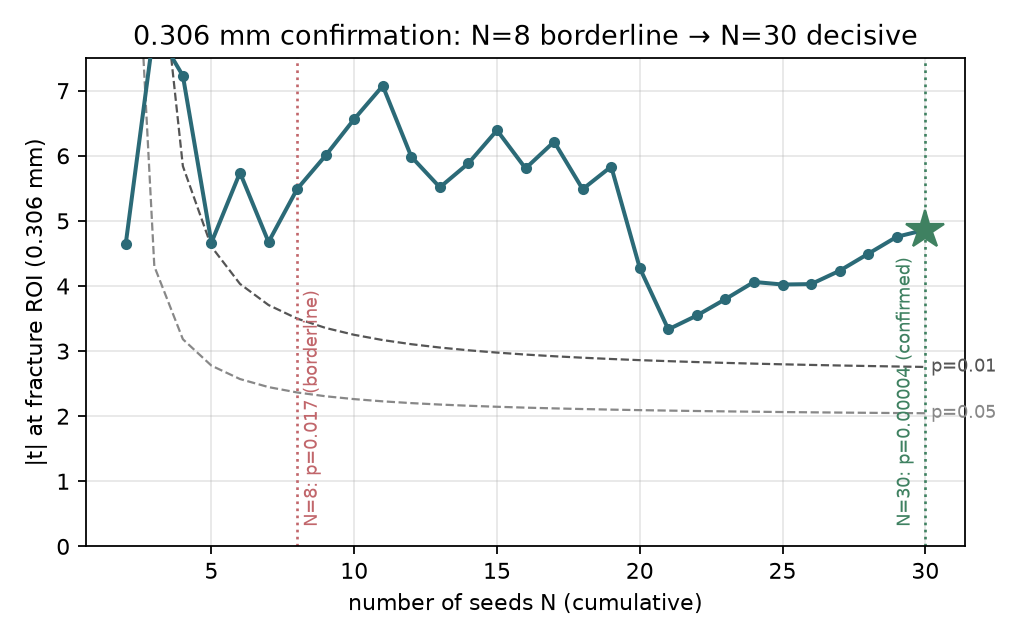
\includegraphics[width=0.60\textwidth]{fig_cl1/confirm.png}
\caption{การรันยืนยันจริง: $|t|$ ของ 0.306~มม.\ เมื่อสะสม seed ถึง $N=30$ (ดาวเขียว) พ้นเส้น $p=0.01$ ชัดเจน}
\end{figure}
\noindent ส่วนภาวะอิ่มตัว (plateau) ระหว่าง 0.54 กับ 1.0~มม.\ \textbf{แยกไม่ออกทางสถิติ} ($p=0.48$) และการแยก
ด้วย ROI-mean ต้องใช้ถึง $\sim$111 seeds --- นำไปสู่ CL-7

\subsection{ความถูกต้องของระเบียบวิธี (CL-2)}
ทดสอบ false-positive rate ด้วย 3 วิธีอิสระ: (1)~\textbf{control-vs-control} (แทน fracture ด้วย control อีกชุด)
ให้ FPR $=5.6$--$5.8\%\approx$ ค่าที่กำหนด $\alpha{=}5\%$; (2)~\textbf{sign-flip permutation} ยืนยันนัยสำคัญ
แบบ non-parametric; (3)~\textbf{spatial} --- พิกเซลนัยสำคัญในลำแสงอยู่ระดับ chance ($\sim$5\%) และเกาะกลุ่มที่ร่อง
$\Rightarrow$ ไม่มี global artifact $\Rightarrow$ \textbf{การตรวจพบเป็นของจริง มิใช่สิ่งประดิษฐ์ของ pipeline}

\begin{figure}[h]\centering
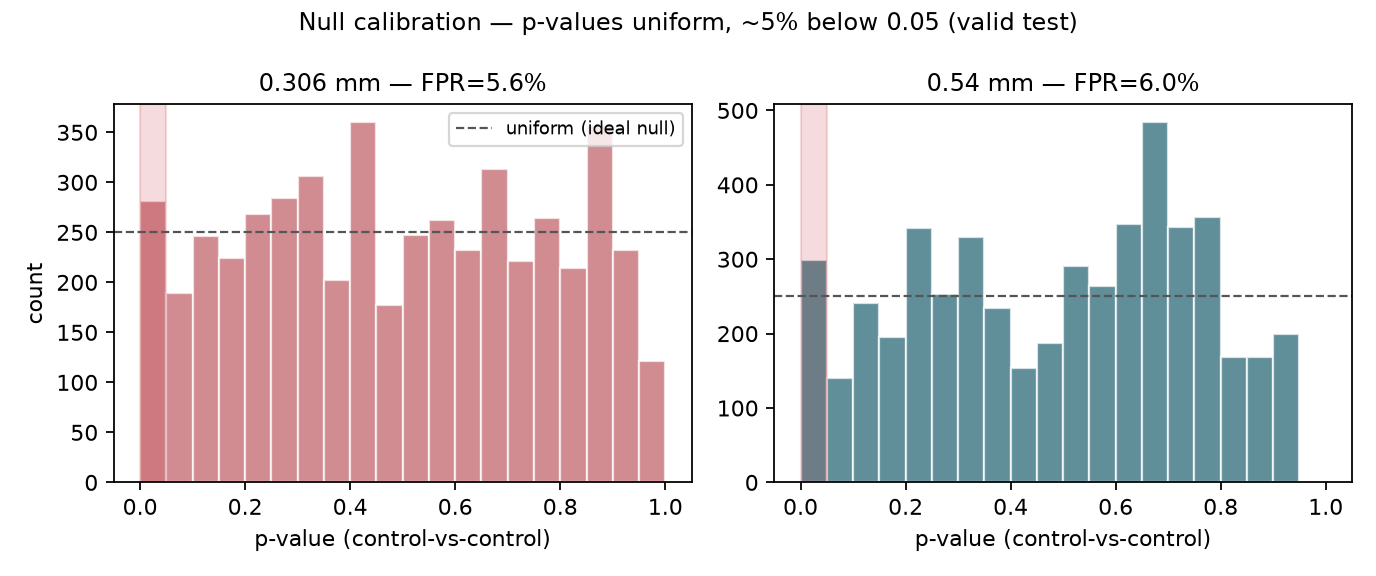
\includegraphics[width=0.86\textwidth]{fig_cl2/calib.png}
\caption{Null calibration: การกระจาย $p$-value ของ control-vs-control เกือบ uniform โดยมีเพียง $\sim$5\% ที่
$p<0.05$ (แถบแดง) = การทดสอบ calibrate ถูกต้อง}
\end{figure}

\subsection{ขอบเขตเชิงกายภาพ --- การอิ่มตัว (CL-7)}
วิเคราะห์ว่า plateau เกิดจาก ROI ขนาดคงที่เจือจางสัญญาณ หรือเป็นการอิ่มตัวจริง โดยวัด\textbf{สัญญาณรวม
(integrated)} ซึ่งจะโตต่อถ้าเป็นเพียงการเจือจาง ผลปรากฏว่า\textbf{สัญญาณรวมก็อิ่มตัว} ($0.54\approx1.0$, $p=0.73$)
$\Rightarrow$ \textbf{plateau เป็นการอิ่มตัวเชิงกายภาพจริง} --- SPR ตรวจ\textbf{การมีอยู่}ของรอยแตกได้ไว
(threshold $\sim$0.3~มม.) แต่\textbf{ความไวต่อความกว้าง}อิ่มตัวเกิน $\sim$0.5~มม.

\begin{figure}[h]\centering
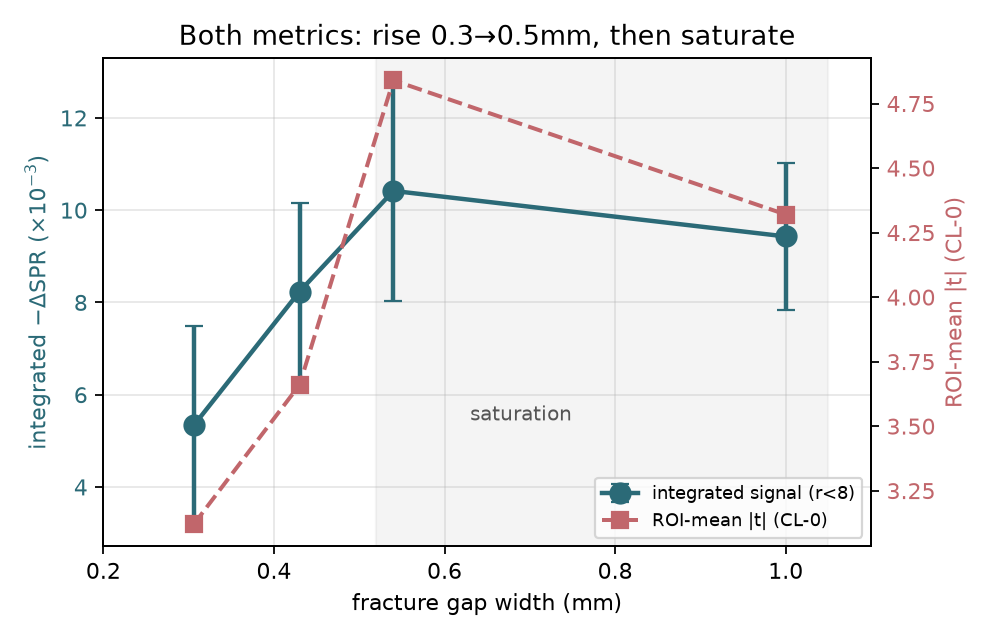
\includegraphics[width=0.62\textwidth]{fig_cl7/integrated.png}
\caption{สัญญาณรวม (แกนซ้าย) และ ROI-mean $|t|$ (แกนขวา) --- ทั้งคู่ขึ้นในช่วง 0.3--0.5~มม.\ แล้วเข้าสู่แถบอิ่มตัว}
\end{figure}

\subsection{การพึ่งพาพลังงาน (CL-3)}
กวาดพลังงาน 40--120~keV (0.54~มม., 10 seeds/พลังงาน) พบหลักฐาน\textbf{สองอย่างที่สอดคล้องกับฟิสิกส์}:
(1)~\textbf{สัญญาณแรงสุดที่ 40~keV} (median $-9.7$ vs $-3.9\times10^{-5}$ เทียบพลังงานสูง, $p=0.0001$) ตามที่
photoelectric ($\mu_{\text{bone}}\propto 1/E^3$) ทำนาย; (2)~\textbf{baseline SPR ลดลง monotonic} ตามพลังงาน
($\rho=-1.00$, $p<0.001$) อย่างไรก็ตามโครงสร้างละเอียด 60--120~keV มี noise สูงที่ $N=10$ (E=60 มี 3 seeds
เป็นบวก $\to$ ไม่ถึงนัยสำคัญ) \textbf{เส้นโค้งเชิงปริมาณจึงยังไม่คมชัด}

\begin{figure}[h]\centering
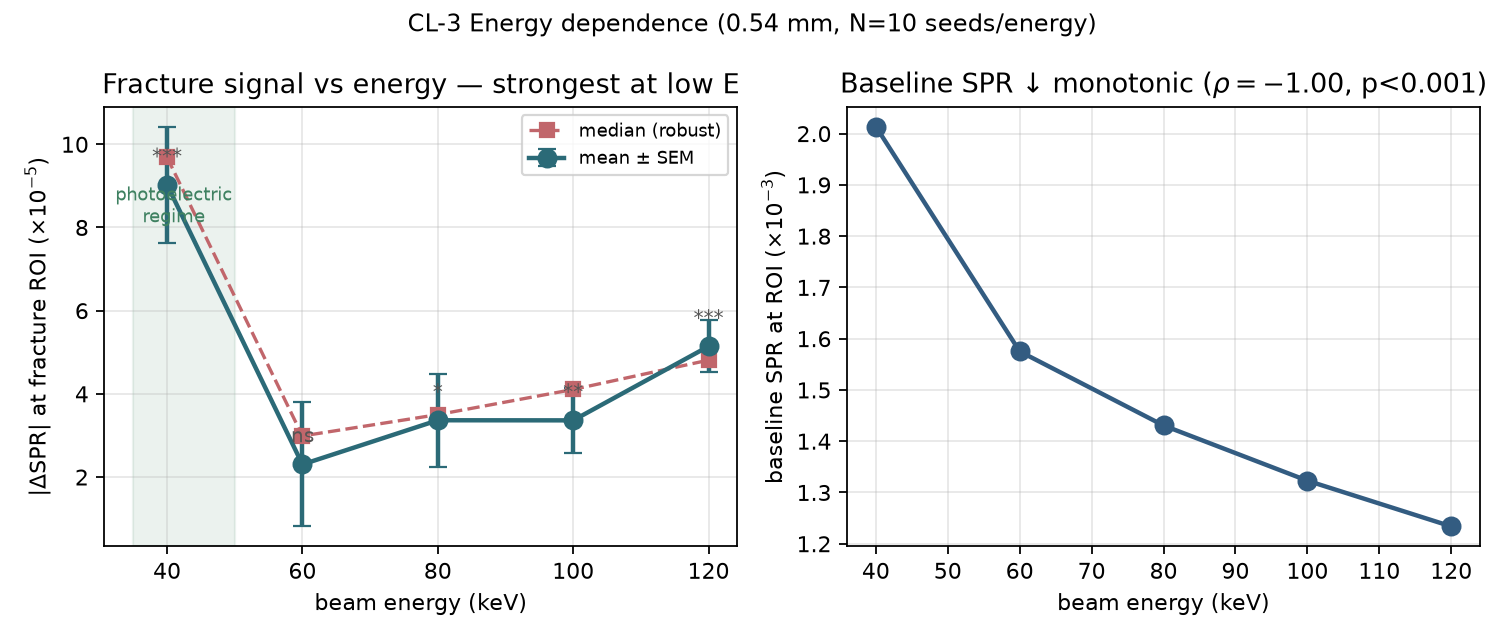
\includegraphics[width=0.88\textwidth]{fig_cl3/energy.png}
\caption{ซ้าย: $|\Delta$SPR$|$ แรงสุดที่ 40~keV (photoelectric regime); ขวา: baseline SPR ลดลง monotonic ตามพลังงาน}
\end{figure}

\subsection{การพึ่งพามุมลำแสง (CL-6)}
กวาดมุม $\pm30^\circ$ (0.54~มม., 10 seeds/มุม, จัดตำแหน่งร่องให้อยู่กลางลำแสงทุกมุม): สัญญาณ\textbf{ตรวจพบได้ทุกมุม}
(เครื่องหมายถูก, 5/6 มีนัยสำคัญ) และ\textbf{$|\Delta$SPR$|$ แรงขึ้น monotonic ตามการเอียง} ($3.4\to6.8\times10^{-5}$
เมื่อ $|\theta|\to30^\circ$) ตรงทิศที่แบบจำลองเส้นทางอากาศทำนาย (เอียงเข้าหา tangential $\to$ air-path ยาวขึ้น)
\textbf{แต่ยังไม่ถึงนัยสำคัญที่ $N=10$} ($p=0.19$) และมุมสุดขอบ $\theta=-30^\circ$ ถูกตัดออก (artifact เชิงเรขาคณิต
จากการเลื่อนวัตถุมากเกิน) $\Rightarrow$ \textbf{สนับสนุนเชิงบ่งชี้ (suggestive) แต่ยังไม่ conclusive}

\begin{figure}[h]\centering
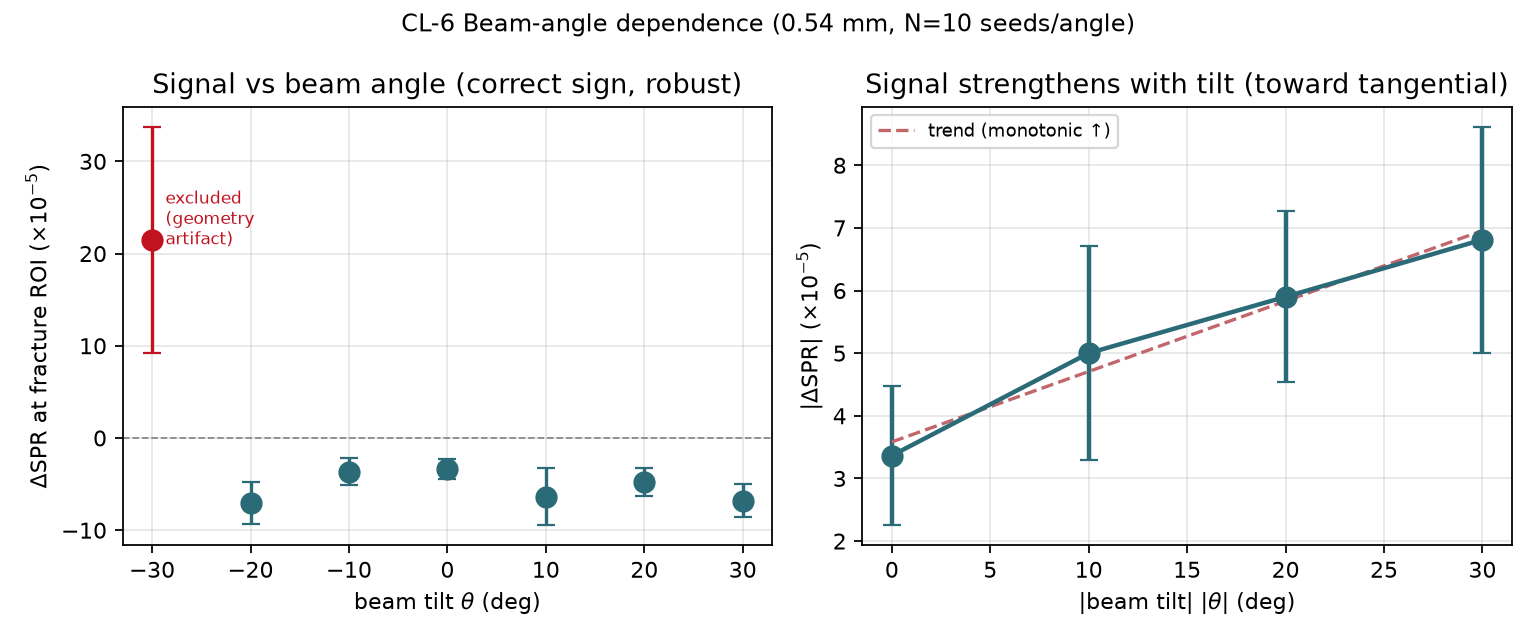
\includegraphics[width=0.88\textwidth]{fig_cl6/angle.png}
\caption{ซ้าย: $\Delta$SPR เทียบมุม ($-30^\circ$ ตัดออก); ขวา: $|\Delta$SPR$|$ เทียบ $|\theta|$ เพิ่มขึ้น monotonic ตามการเอียง}
\end{figure}

% ================= 4. SYNTHESIS =================
\section{สังเคราะห์ --- 6 เสาหลักของ Phase 1}
\renewcommand{\arraystretch}{1.3}
\small
\begin{longtable}{c l l c}
\rowcolor{theme}\color{white}\textbf{CL} & \color{white}\textbf{เสา / คำถาม} & \color{white}\textbf{ผลลัพธ์หลัก} & \color{white}\textbf{สถานะ} \\
\midrule
\endhead
CL-0 & Detection --- เจอสัญญาณไหม & ตรวจพบครบ 4 ขนาด ($p<0.02$), เครื่องหมายถูก & \pgood \\
\rowcolor{softgray}
CL-1 & Robustness \& power --- มั่นคงไหม & CI ตัด 0 ทุกขนาด; 0.306~มม.\ ยืนยัน $p=4\!\times\!10^{-5}$ & \pgood \\
CL-2 & Validity --- artifact ไหม & false-positive rate $\approx5\%$; ไม่มี global artifact & \pgood \\
\rowcolor{softgray}
CL-7 & Physical bound --- plateau คืออะไร & อิ่มตัวเชิงกายภาพ ($>0.5$~มม.); ไวต่อ ``การมีอยู่'' & \pgood \\
CL-3 & Energy --- ตามฟิสิกส์ไหม & แรงสุดที่ E ต่ำ + baseline monotonic; noisy ที่ $N{=}10$ & \pgood \\
\rowcolor{softgray}
CL-6 & Geometry --- ตามเรขาคณิตไหม & robust ทุกมุม + แรงขึ้นตามการเอียง; ไม่ conclusive & \ppart \\
\bottomrule
\end{longtable}
\normalsize
\begin{verdictbox}{ข้อสรุปรวม Phase 1 (ซื่อตรง)}
\textbf{สมมติฐานหลักได้รับการสนับสนุนอย่างแข็งแรง:} SPR มีลายเซ็นรอยแตกที่\textbf{จริง, ยืนยันเชิงสถิติ,
ไม่ใช่ artifact, และมีที่มาเชิงฟิสิกส์} ตรวจพบได้ถึง $\sim$0.3~มม. --- 4 เสาแรก (detection, robustness, validity,
physical bound) \textbf{มั่นคง}; เสาเชิงกลไก (energy) \textbf{สนับสนุน}; เสาเชิงเรขาคณิต (geometry)
\textbf{บ่งชี้แต่ยังไม่ conclusive}. ค้นพบที่สำคัญคือ \textbf{SPR เหมาะกับการ ``ตรวจพบ'' รอยแตกมากกว่าการ
``วัดความกว้าง''} (สัญญาณอิ่มตัวเกิน $\sim$0.5~มม.). โดยรวม \textbf{เป็น proof-of-concept ที่มั่นคงพอสำหรับ
การพัฒนาต่อใน Phase 2}
\end{verdictbox}

% ================= 5. LIMITATIONS =================
\section{ข้อจำกัด (ระบุอย่างซื่อตรง)}
\begin{itemize}
  \item \textbf{ขอบเขตของ observable:} SPR ไวต่อ ``การมีอยู่'' ของรอยแตก แต่\textbf{อิ่มตัวเชิงความกว้าง}เกิน
        $\sim$0.5~มม.\ (CL-7) --- ไม่เหมาะกับการวัดขนาดรอยแตกใหญ่
  \item \textbf{สถิติของการทดสอบเชิงกลไก:} CL-3 (พลังงาน) และ CL-6 (มุม) รันที่ $N=10$ ซึ่ง noise สูง ---
        แนวโน้มตรงทิศที่ทำนายแต่\textbf{ยังไม่ถึงนัยสำคัญเชิงปริมาณ}; ต้องเพิ่มเป็น $N=20$--$30$
  \item \textbf{ขีดจำกัดเชิงเรขาคณิต:} ที่มุมเอียงมาก (CL-6, $\theta=-30^\circ$) การเลื่อนวัตถุเพื่อจัดร่องให้
        กลางลำแสงมากเกินไปทำให้เกิด artifact --- ต้องออกแบบการหมุนรอบจุดร่องโดยตรง
  \item \textbf{ความสมจริงของแบบจำลอง:} ยังเป็นฉากรับอุดมคติ (ไม่รวมประสิทธิภาพเชิงพลังงาน, จุดกระเจิงในฉากรับ),
        ลำแสง mono (ไม่ใช่สเปกตรัมจริง), รอยแตกตำแหน่ง/ทิศเดียว, ยังไม่เทียบกับข้อมูลภาพจริง
\end{itemize}

% ================= 6. CONCLUSIONS =================
\section{สรุปและงานถัดไป (Phase 2)}
งาน Phase 1 ได้พัฒนา\textbf{ระเบียบวิธีที่ถูกต้อง}สำหรับตรวจวัดลายเซ็นการกระเจิงจากรอยแตก (matched control +
multi-seed significance) ซึ่งเผยสัญญาณที่การเทียบแบบไร้เดียงสามองไม่เห็น และแสดง\textbf{หลักฐานเชิงประจักษ์}
ว่าลายเซ็น SPR จากรอยแตกระดับต่ำกว่ามิลลิเมตรตรวจพบได้อย่างมีนัยสำคัญ ยืนยันเชิงสถิติ ไม่ใช่ artifact และ
มีที่มาเชิงฟิสิกส์ --- เป็นฐานที่มั่นคงสำหรับ:
\begin{enumerate}
  \item \textbf{ยืนยันเชิงกลไกให้สมบูรณ์:} รัน CL-3/CL-6 ที่ $N=20$--$30$ + ช่วงมุมกว้างขึ้น (จนถึง tangential)
        เพื่อยกแนวโน้มพลังงาน/มุมให้ถึงนัยสำคัญเชิงปริมาณ
  \item \textbf{เพิ่มความสมจริง:} ฉากรับเชิงจริง, สเปกตรัมพลังงาน (kVp จริง + filtration), การเทียบกับภาพจริง
  \item \textbf{ขยายขอบเขต:} ตำแหน่ง/ทิศทางรอยแตกอื่น, บริเวณกายวิภาคอื่น, และ optimization ของพารามิเตอร์
        (พลังงาน, collimation, air-gap, ความละเอียด) เพื่อ CNR สูงสุด
\end{enumerate}

\vfill
\noindent{\color{theme!45}\rule{\linewidth}{0.4pt}}\\
{\small\color{ink} รายงานฉบับสมบูรณ์ Phase 1. ผลและรูปทั้งหมดคำนวณจากการรันจริง (repository
\code{intraprasart/GATE-Xray-pelvis-SPR}). รายงานย่อยรายเสา (CL-0…CL-7) และไฟล์นี้เผยแพร่ที่
https://wwaxray.baanwit.com/doc/report/}

\end{document}
